% 我们提出的算法(pseudo code)
% \begin{frame}{Offline-FAST}
% Former work towards fairness:

% \begin{figure}
%     \centering
%     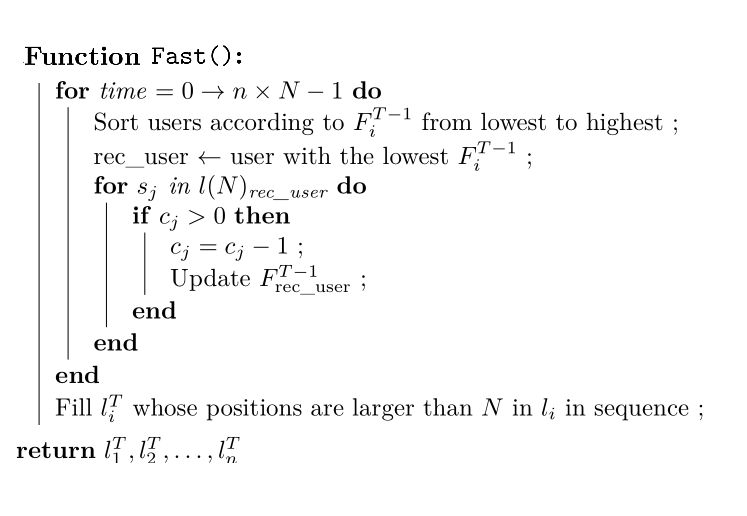
\includegraphics[width=1\textwidth]{img/a1.png}
%     \label{Algo1}
% \end{figure}
% \begin{figure}
%     \centering
%     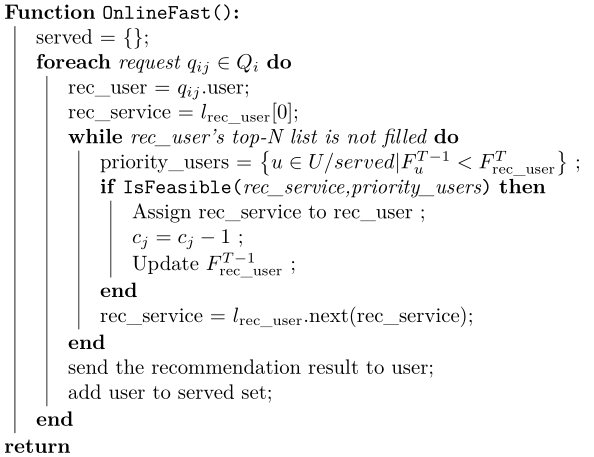
\includegraphics[width=0.8\textwidth]{img/a2.png}
%     \label{Algo2}
% \end{figure}
% \end{frame}

\begin{frame}{Online-FAST}
\begin{figure}[H]
  \centering
  \subfigure{
    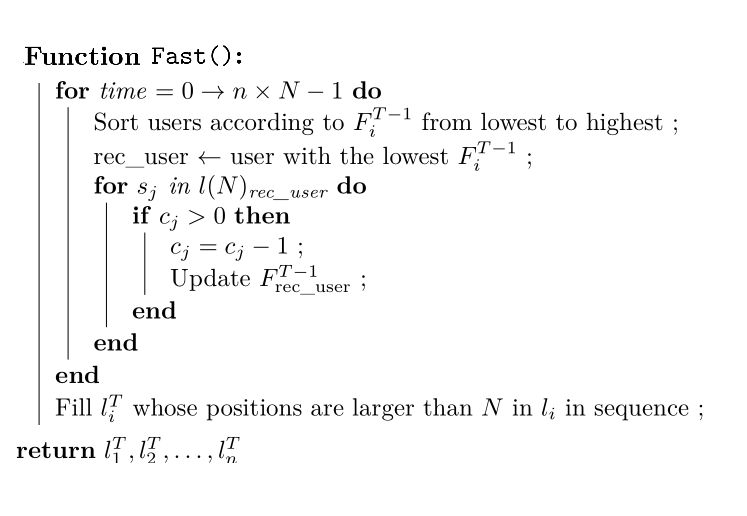
\includegraphics[width=0.45\textwidth]{img/a1.png}}
  \hspace{0.2in} % 两图片之间的距离
  \subfigure{
    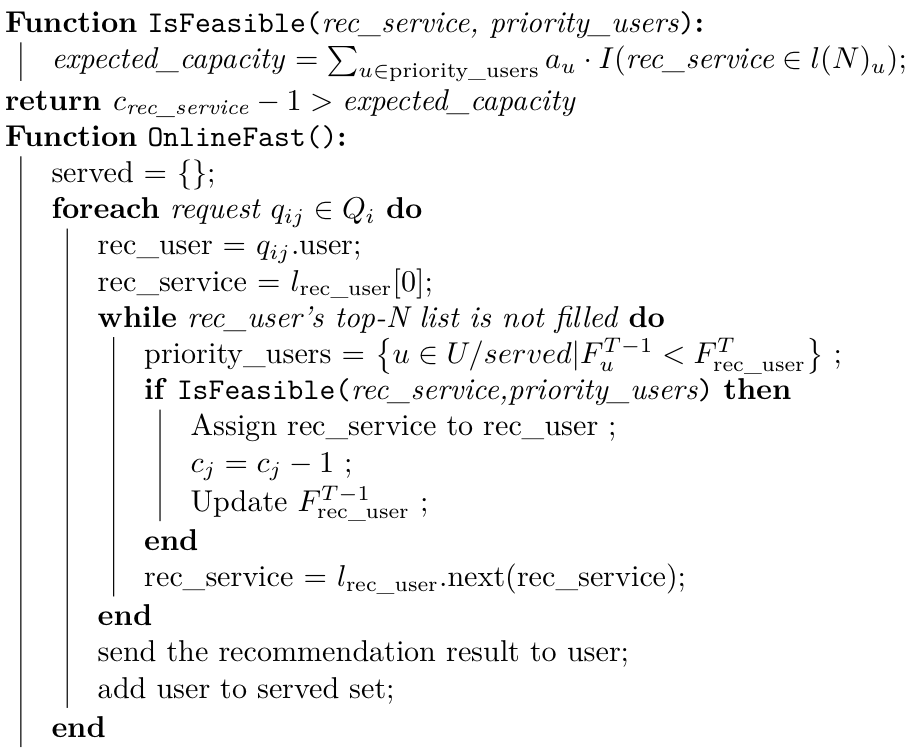
\includegraphics[width=0.45\textwidth]{img/algorithm2_new.png}}
   \caption{Comparing 2 algorithms}
\end{figure}

By using \texttt{IsFeasible} as a heuristic, we avoid the high computational cost of sorting and eliminate the dependency on future requests in Offline-FAST.
 
\end{frame}
